\chapter{Analisi}

\section{Descrizione e requisiti}

Il software mira alla costruzione di una versione virtuale del famoso gioco da tavolo “Monopoly”. 
Quest’ultimo è un gioco di società nel quale più giocatori muovono a turno le proprie pedine su un tabellone 
composto da caselle; la maggior parte di queste sono proprietà: ovvero terreni acquistabili dai giocatori.
Lo scopo del gioco è di creare un monopolio, aumentando i beni o il denaro posseduto. 
Durante la partita i giocatori possono acquistare le proprietà capitandovi sopra e pagando una somma alla banca.
Una volta acquistate il giocatore potrà anche decidere se eventualmente migliorare le proprietà.
I giocatori si scambiano denaro a vicenda sotto 
forma di pagamenti. Quando un giocatore capita su una proprietà di un altro giocatore è costretto a pagare
a questo una somma di denaro. 
L’obiettivo è mandare gli altri giocatori in bancarotta, vince l’ultimo giocatore rimasto. 
Il software permetterà di creare e giocare un partita con un determinato numero di giocatori dallo 
stesso terminale.



\subsection*{Requisiti funzionali}
\begin{itemize}
    \item Il gioco potrà essere giocato su uno stesso dispositivo da un minimo di 2 giocatori ed un massimo di 6.
	\item Il giocatore potrà tirare i dadi per far muovere la propria pedina sul tabellone.
	\item Durante il proprio turno ciascun giocatore avrà la possibilità di acquistare la proprietà sulla quale 
    si trova la sua pedina, se la proprietà non appartiene a nessuno, altrimenti potrà pagare l’affitto al proprietario.
    \item Sul tabellone saranno presenti delle caselle speciali con effetti specifici sulla partita
    \item Nel corso della partita un giocatore, quando capita sulle sue proprietà, le potrà migliorare spendendo
    del denaro per posizionare delle case che elevano il costo dell’affitto.
    \item Durante il proprio turno, se lo desidera, il giocatore potrà vendere alla banca 
    le proprietà o eventuali case presenti su esse.
\end{itemize}


\subsection*{Requisiti non funzionali}
\begin{itemize}
    \item 
    Monopoly dovrà permettere agli utenti di aggiungere e 
    modificare gli effetti speciali del gioco in facilità e senza toccare il codice
    \item \b NON LO INSERIREI \b salvare su file lo storico dei risultati delle partite precedenti
    \item Monopoly potrà essere giocato attraverso un'interfaccia grafica
    che dovrà essere in grado di adattarsi alle dimensioni di vari schermi
    \item 
    Monopoly dovrà permettere agli utenti di alterare in facilità la 
    configurazione del gioco (impostazioni, struttura del tabellone e caselle che lo compongono)
    \item \b NON LO INSERIREI \b rendere l’applicazione portabile su più SO
\end{itemize}

\section{Modello del dominio}
Il sistema (TurnationManager) deve gestire l’avvicendarsi dei vari turni dei giocatori. 
A ogni giocatore (Player) viene concesso periodicamente il proprio turno d’azione sulla base di una rotazione ciclica. 
Durante il turno il giocatore tira i dadi e muove sul tabellone (Board) la propria pedina (Pawn) finendo sempre su una casella (Tile).
Questa casella può essere una proprietà (Property) oppure una casella speciale (Special), 
e sulla base di ciò cambia radicalmente l’interazione dell’utente. 
Se la pedina capita su una proprietà che non è ancora posseduta da alcun giocatore allora 
il giocatore può chiedere alla banca (Bank) di acquistarla pagando dei soldi. 
Se invece la proprietà era già stata comprata in precedenza da un altro giocatore allora si 
deve pagare l'affitto al proprietario. 
Se la pedina del giocatore capita su una sua proprietà  
può decidere se migliorarla aggiungendo case e pagando dei soldi alla banca. 
Oppure se desidera può vendere la proprietà, in tal caso riceverà dei soldi dalla banca e la proprietà ritornerà
disponibile all'acquisto.
Se capita su una casella speciale invece si attiverà un effetto caratteristico della casella (Effect)
che avrà ripercussioni sullo svolgimento del gioco 
(guadagno/perdita denaro, saltare un determinato numero di turni, affrontare sfide).
Una volta che il giocatore avrà svolto tutte le azioni obbligatorie potrà decidere di terminare il proprio turno. 
Fatto questo se il suo saldo è in negativo perde la partita e tutte le sue proprietà tornano disponibili per l’acquisto. 




\begin{figure}[H]
    \centering
    \makebox[1.0\textwidth]{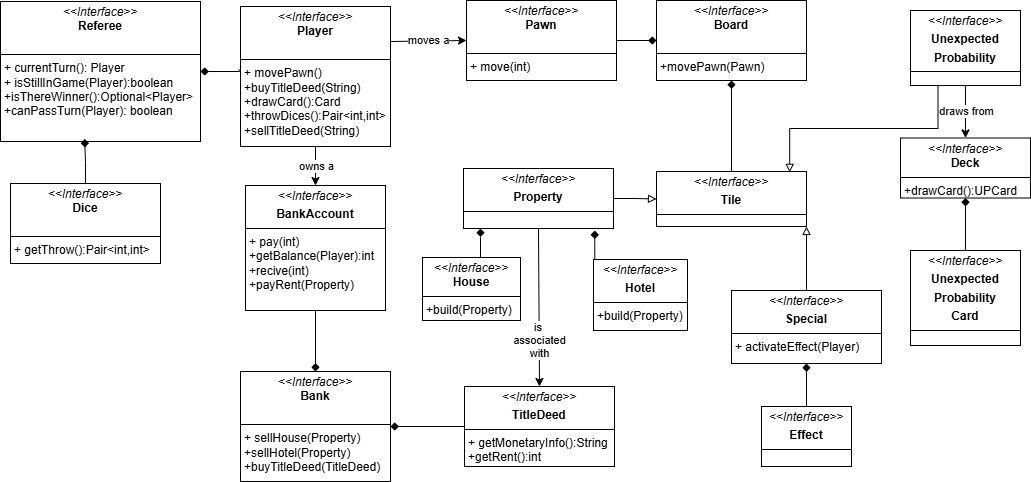
\includegraphics[width=1.3\textwidth]{img/entity_diagram.png}}	
    \caption{Schema UML dell'analisi del problema, con rappresentate le entità principali ed i rapporti fra loro}
	\label{img:entity_diagram}
\end{figure}
